The given equation of the line in parametric form:
\begin{align}
\vec{x} = \vec{A} + \lambda \vec{m} 
\end{align}
where,
\begin{align}
\vec{A} = \myvec{3\\1}
\end{align}
\begin{align}
\vec{m} = \myvec{1\\-1}
\end{align}
If $\vec{x}$ be the point of intersection, 
\begin{align}
	\norm{\vec{x}-\vec{B}}=3 
\end{align}
\begin{align}
	\norm{\vec{A}+\lambda \vec{m}-\vec{B}}=3 
\end{align}
\begin{align}
	(\vec{A}+\lambda\vec{m}-\vec{B})^T (\vec{A}+\lambda\vec{m}-\vec{B}) =9
\end{align}
\begin{align}
	[(\vec{A}-\vec{B})^T\vec{m} = \vec{m}^T(\vec{A}-\vec{B})]
\end{align}
\begin{align}
	\norm{\vec{m}}^2 \lambda^2+ \sbrak{2(\vec{A}-\vec{B})^T\vec{m})} \lambda + \norm{\vec{A}-\vec{B}}^2=9
\end{align}
\begin{align}
	2\lambda^2+ 10\lambda+8=0 
\end{align} 
\begin{align}
	\lambda=-4,  \lambda=-1 
\end{align} 
The point of intersection,
\begin{align}
	\boxed{\therefore \vec{x}=\myvec{-1\\5} or \myvec{2\\2}}
\end{align} 
The direction vector, 
    \begin{align}
		\vec{v} = \vec{B}-\vec{x}
	\end{align}
	\begin{align}
		\boxed{\vec{v} = \myvec{0 \\ -3} or \myvec{-3 \\ 0}}
	\end{align}
%See Fig. \ref{eq:solutions/line_plane/53/}
%
%\begin{figure}[h]
%    \centering
%    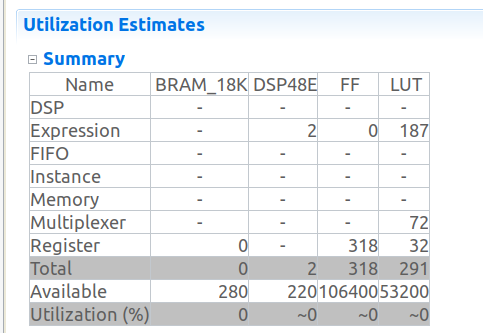
\includegraphics[width=0.37\textwidth]{./solutions/line_plane/53/Test/1.png}
%\caption{}
%\label{eq:solutions/line_plane/53/}
%\end{figure}
